\section{Neural Networks and Deep Learning}
\subsection{Python Basics with numpy (optional)}

Welcome to your first (Optional) programming exercise of the deep learning specialization. This exercise gives you a brief introduction to Python. Even if you've used Python before, this will help familiarize you with functions we'll need. In this assignment you will:
\begin{itemize}
\item Learn how to use numpy.
\item Implement some basic core deep learning functions such as the softmax, sigmoid, dsigmoid, etc...
\item Learn how to handle data by normalizing inputs and reshaping images.
\item Recognize the importance of vectorization.
\item Understand how python broadcasting works.
\end{itemize}

This assignment prepares you well for the upcoming assignment. Take your time to complete it and make sure you get the expected outputs when working through the different exercises. In some code blocks, you will find a "\#GRADED FUNCTION: functionName" comment. Please do not modify it. After you are done, submit your work and check your results. You need to score 70\% to pass. Good luck :) !

Let's get started!

\subsubsection{About iPython Notebooks}

iPython Notebooks are interactive coding environments embedded in a webpage. You will be using iPython notebooks in this class. You only need to write code between the \#\#\# START CODE HERE \#\#\# and \#\#\# END CODE HERE \#\#\# comments. After writing your code, you can run the cell by either pressing ``SHIFT"+``ENTER" or by clicking on ``Run Cell" (denoted by a play symbol) in the upper bar of the notebook.

We will often specify ``($\approx$ lines of code)'' in the comments to tell you about how much code you need to write. It is just a rough estimate, so don't feel bad if your code is longer or shorter.


{\textbf {Exercise}}: Set test to ``Hello World" in the cell below to print ``Hello World" and run the two code below.
\begin{minted}{python}
### START CODE HERE ### (≈ 1 line of code)
test = "Hello World"
### END CODE HERE ###

print ("test: " + test)

#output
test: Hello World
\end{minted}

{\textbf {What you need to remember}}:
\begin{itemize}
\item Run your cells using SHIFT+ENTER (or ``Run cell")
\item Write code in the designated areas using Python 3 only
\item Do not modify the code outside of the designated areas
\end{itemize}

\subsubsection{Building basic functions with numpy}

Numpy is the main package for scientific computing in Python. It is maintained by a large community (www.numpy.org). In this exercise you will learn several key numpy functions such as np.exp, np.log, and np.reshape. You will need to know how to use these functions for future assignments.


\subsubsubsection{sigmoid function, np.exp()}

Before using np.exp(), you will use math.exp() to implement the sigmoid function. You will then see why np.exp() is preferable to math.exp().

{\textbf {Exercise}}: Build a function that returns the sigmoid of a real number x. Use math.exp(x) for the exponential function.


{\textbf {Reminder}}: $sigmoid(x) = \frac{{\rm{1}}}{{{\rm{1 + }}{e^{ - x}}}}$ is sometimes also known as the logistic function. It is a non-linear function used not only in Machine Learning (Logistic Regression), but also in Deep Learning.
\begin{figure}[h]
\begin{center}
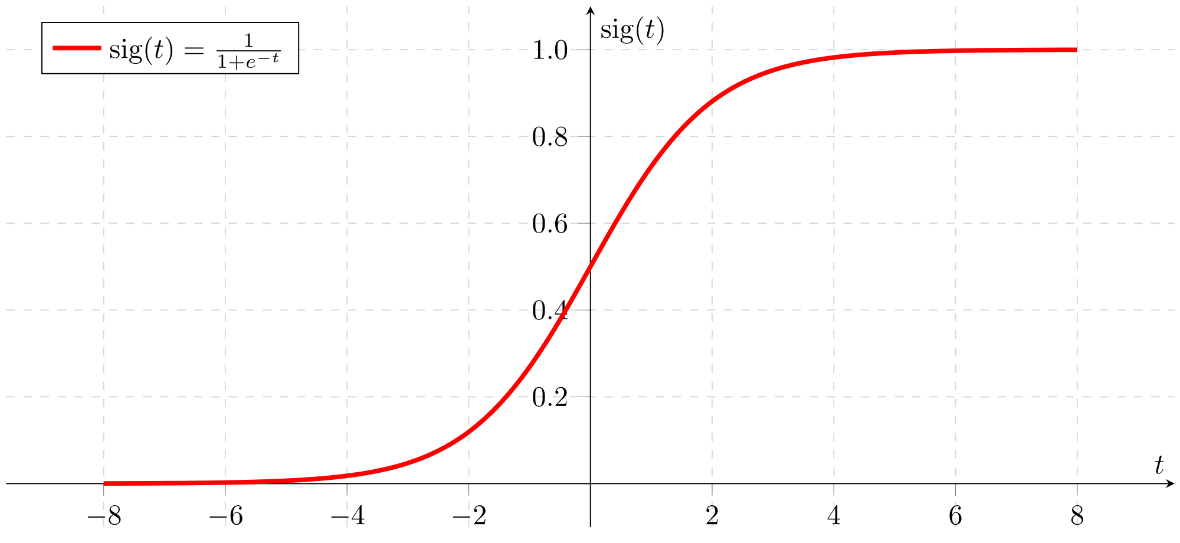
\includegraphics[width=0.8\textwidth]{course1/sigmoid}
\end{center}
\caption{$sigmoid(t) = \frac{{\rm{1}}}{{{\rm{1 + }}{e^{ - t}}}}$}
\end{figure}

To refer to a function belonging to a specific package you could call it using package\_name.function(). Run the code below to see an example with math.exp().

\begin{minted}{python}
# GRADED FUNCTION: basic_sigmoid
import math

def basic_sigmoid(x):
    """
    Compute sigmoid of x.

    Arguments:
    x -- A scalar

    Return:
    s -- sigmoid(x)
    """
    
    ### START CODE HERE ### (≈ 1 line of code)
    s = 1/(1+math.exp(-x))
    ### END CODE HERE ###
    
    return s
\end{minted}

Actually, we rarely use the ``math" library in deep learning because the inputs of the functions are real numbers. In deep learning we mostly use matrices and vectors. This is why numpy is more useful.

In fact, if $ x = (x_1, x_2, ..., x_n)$ is a row vector then $np.exp(x)$ will apply the exponential function to every element of x. The output will thus be: $np.exp(x) = (e^{x_1}, e^{x_2}, ..., e^{x_n})$
\begin{minted}{python}
import numpy as np

# example of np.exp
x = np.array([1, 2, 3])
print(np.exp(x)) # result is (exp(1), exp(2), exp(3))

#output
[  2.71828183   7.3890561   20.08553692]
\end{minted}

Furthermore, if x is a vector, then a Python operation such as $s = x + 3$ or $s = \frac{1}{x}$ will output s as a vector of the same size as x.
\begin{minted}{python}
# example of vector operation
x = np.array([1, 2, 3])
print (x + 3)

#output
[4 5 6]
\end{minted}

{\textbf {Exercise}}: Implement the sigmoid function using numpy. 

{\textbf {Instructions}}: x could now be either a real number, a vector, or a matrix. The data structures we use in numpy to represent these shapes (vectors, matrices...) are called numpy arrays. You don't need to know more for now.

For x $\in$ $\mathbb{R}^n$ ,
\begin{equation}
sigmoid(x) = sigmoid\begin{pmatrix}
    x_1  \\
    x_2  \\
    ...  \\
    x_n  \\
\end{pmatrix} = \begin{pmatrix}
    \frac{1}{1+e^{-x_1}}  \\
    \frac{1}{1+e^{-x_2}}  \\
    ...  \\
    \frac{1}{1+e^{-x_n}}  \\
\end{pmatrix}
\end{equation}

\begin{minted}{python}
# GRADED FUNCTION: sigmoid
import numpy as np # this means you can access numpy functions by writing np.function() instead of numpy.function()

def sigmoid(x):
    """
    Compute the sigmoid of x

    Arguments:
    x -- A scalar or numpy array of any size

    Return:
    s -- sigmoid(x)
    """
    
    ### START CODE HERE ### (≈ 1 line of code)
    s = 1/(1+np.exp(-x))
    ### END CODE HERE ###
    
    return s
\end{minted}

\begin{minted}{python}
x = np.array([1,2,3])
sigmoid(x)

#output
array([ 0.73105858,  0.88079708,  0.95257413])
\end{minted}

\subsubsubsection{Sigmoid gradient}

As you've seen in lecture, you will need to compute gradients to optimize loss functions using backpropagation. Let's code your first gradient function.

{\textbf {Exercise}}: Implement the function sigmoid\_grad() to compute the gradient of the sigmoid function with respect to its input x. The formula is: 
\begin{equation}
sigmoid\_derivative(x) = \sigma'(x) = \sigma(x) (1 - \sigma(x))
\end{equation}

You often code this function in two steps:
\begin{itemize}
\item[1.] Set s to be the sigmoid of x. You might find your sigmoid(x) function useful.
\item[2.] Compute $\sigma'(x) = s(1-s)$
\end{itemize}


\begin{minted}{python}
# GRADED FUNCTION: sigmoid_derivative
def sigmoid_derivative(x):
    """
    Compute the gradient (also called the slope or derivative) of the sigmoid function with respect to its input x.
    You can store the output of the sigmoid function into variables and then use it to calculate the gradient.
    
    Arguments:
    x -- A scalar or numpy array

    Return:
    ds -- Your computed gradient.
    """
    
    ### START CODE HERE ### (≈ 2 lines of code)
    s = 1/(1+np.exp(-x))
    ds = s*(1-s)
    ### END CODE HERE ###
    
    return ds
\end{minted}



\subsubsubsection{Reshaping arrays}
Two common numpy functions used in deep learning are \href{https://docs.scipy.org/doc/numpy/reference/generated/numpy.ndarray.shape.html}{np.shape} and \href{https://docs.scipy.org/doc/numpy/reference/generated/numpy.reshape.html}{np.reshape()}. 
\begin{itemize}
\item X.shape is used to get the shape (dimension) of a matrix/vector X. 
\item X.reshape(...) is used to reshape X into some other dimension. 
\end{itemize}

For example, in computer science, an image is represented by a 3D array of shape $(length, height, depth = 3)$. However, when you read an image as the input of an algorithm you convert it to a vector of shape $(length*height*3, 1)$. In other words, you ``unroll", or reshape, the 3D array into a 1D vector.

\begin{figure}[h]
\begin{center}
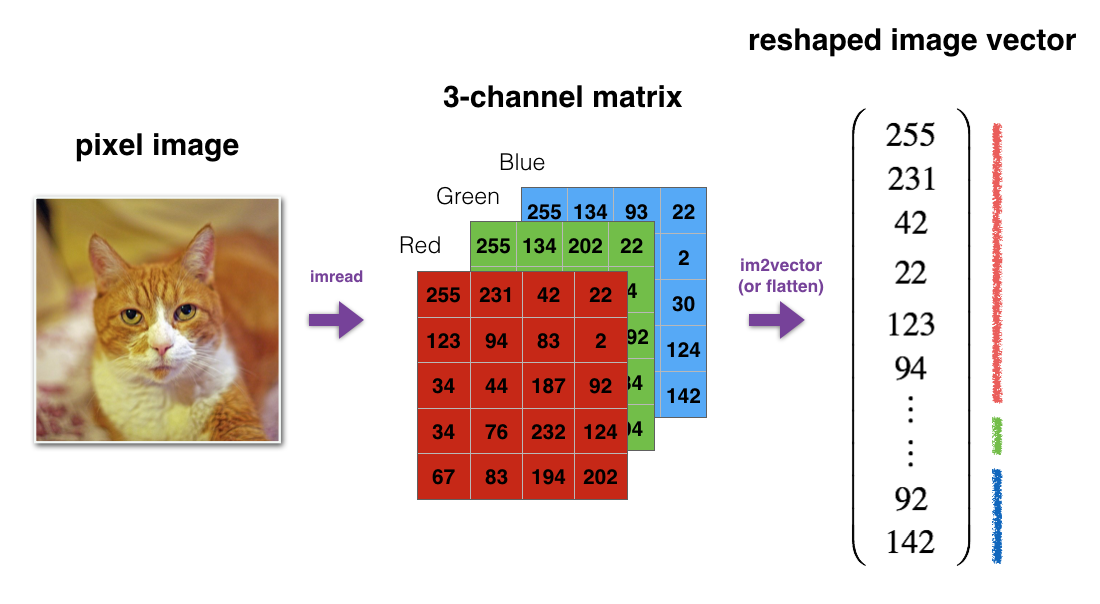
\includegraphics[width=0.8\textwidth]{course1/image2vector}
\end{center}
\caption{Reshape image a vector}
\end{figure}

{\textbf {Exercise}}: Implement ``image2vector()'' that takes an input of shape (length, height, 3) and returns a vector of shape (length\*height\*3, 1). For example, if you would like to reshape an array v of shape (a, b, c) into a vector of shape (a*b,c) you would do:
\begin{minted}{python}
v = v.reshape((v.shape[0]*v.shape[1], v.shape[2])) # v.shape[0] = a ; v.shape[1] = b ; v.shape[2] = c
\end{minted}

Please don't hardcode the dimensions of image as a constant. Instead look up the quantities you need with ``image.shape[0]'', etc. 

\begin{minted}{python}
# GRADED FUNCTION: image2vector
def image2vector(image):
    """
    Argument:
    image -- a numpy array of shape (length, height, depth)
    
    Returns:
    v -- a vector of shape (length*height*depth, 1)
    """
    
    ### START CODE HERE ### (≈ 1 line of code)
    v = image.reshape((image.shape[0]*image.shape[1]*image.shape[2]),1)
    ### END CODE HERE ###
    
    return v
\end{minted}


\subsubsubsection{Normalizing rows}

Another common technique we use in Machine Learning and Deep Learning is to normalize our data. It often leads to a better performance because gradient descent converges faster after normalization. Here, by normalization we mean changing x to $ \frac{x}{\| x\|} $ (dividing each row vector of x by its norm).

For example, if 
\begin{equation}
x = 
\begin{bmatrix}
    0 & 3 & 4 \\
    2 & 6 & 4 \\
\end{bmatrix}
\end{equation}
then 
\begin{equation}
\| x\| = np.linalg.norm(x, axis = 1, keepdims = True) = \begin{bmatrix}
    5 \\
    \sqrt{56} \\
\end{bmatrix}
\end{equation}
and
\begin{equation}
x\_normalized = \frac{x}{\| x\|} = \begin{bmatrix}
    0 & \frac{3}{5} & \frac{4}{5} \\
    \frac{2}{\sqrt{56}} & \frac{6}{\sqrt{56}} & \frac{4}{\sqrt{56}} \\
\end{bmatrix}
\end{equation}
Note that you can divide matrices of different sizes and it works fine: this is called broadcasting and you're going to learn about it in part \ref{Broadcasting}.

{\textbf {Exercise}}:  Implement normalizeRows() to normalize the rows of a matrix. After applying this function to an input matrix x, each row of x should be a vector of unit length (meaning length 1).

\begin{minted}{python}
# GRADED FUNCTION: normalizeRows
def normalizeRows(x):
    """
    Implement a function that normalizes each row of the matrix x (to have unit length).
    
    Argument:
    x -- A numpy matrix of shape (n, m)
    
    Returns:
    x -- The normalized (by row) numpy matrix. You are allowed to modify x.
    """
    
    ### START CODE HERE ### (≈ 2 lines of code)
    # Compute x_norm as the norm 2 of x. Use np.linalg.norm(..., ord = 2, axis = ..., keepdims = True)
    x_norm = np.linalg.norm(x,axis=1,keepdims=True)
    
    # Divide x by its norm.
    x = x/x_norm
    ### END CODE HERE ###

    return x
\end{minted}

\begin{minted}{python}
x = np.array([
    [0, 3, 4],
    [1, 6, 4]])
print("normalizeRows(x) = " + str(normalizeRows(x)))

#output
normalizeRows(x) = [[ 0.          0.6         0.8       ]
 [ 0.13736056  0.82416338  0.54944226]]
\end{minted}

{\textbf {Note}}: In normalizeRows(), you can try to print the shapes of x\_norm and x, and then rerun the assessment. You'll find out that they have different shapes. This is normal given that x\_norm takes the norm of each row of x. So x\_norm has the same number of rows but only 1 column. So how did it work when you divided x by x\_norm? This is called broadcasting and we'll talk about it now!



\subsubsubsection{Broadcasting and the softmax function}\label{Broadcasting}

A very important concept to understand in numpy is "broadcasting". It is very useful for performing mathematical operations between arrays of different shapes. For the full details on broadcasting, you can read the official \href{http://docs.scipy.org/doc/numpy/user/basics.broadcasting.html}{broadcasting documentation}.

{\textbf {Exercise}}: Implement a softmax function using numpy. You can think of softmax as a normalizing function used when your algorithm needs to classify two or more classes. You will learn more about softmax in the second course of this specialization.

{\textbf {Instructions}}:
\begin{itemize}
\item for  x $\in$ $\mathbb{R}^{1\times n}$ , 
\begin{equation}
\begin{aligned}
softmax(x) &= softmax(\begin{bmatrix}
    x_1  &&
    x_2 &&
    ...  &&
    x_n  
\end{bmatrix}) \\
&= \begin{bmatrix}
     \frac{e^{x_1}}{\sum_{j}e^{x_j}}  &&
    \frac{e^{x_2}}{\sum_{j}e^{x_j}}  &&
    ...  &&
    \frac{e^{x_n}}{\sum_{j}e^{x_j}} 
\end{bmatrix} 
\end{aligned}
\end{equation}
\item for a matrix $ x \in \mathbb{R}^{m \times n} $,  $x_{ij}$ maps to the element in the $i^{th}$ row and $j^{th}$ column of $x$, thus we have: 
\begin{equation}
\begin{aligned}
softmax(x) &= softmax\begin{bmatrix}
    x_{11} & x_{12} & x_{13} & \dots  & x_{1n} \\
    x_{21} & x_{22} & x_{23} & \dots  & x_{2n} \\
    \vdots & \vdots & \vdots & \ddots & \vdots \\
    x_{m1} & x_{m2} & x_{m3} & \dots  & x_{mn}
\end{bmatrix} \\
&= \begin{bmatrix}
    \frac{e^{x_{11}}}{\sum_{j}e^{x_{1j}}} & \frac{e^{x_{12}}}{\sum_{j}e^{x_{1j}}} & \frac{e^{x_{13}}}{\sum_{j}e^{x_{1j}}} & \dots  & \frac{e^{x_{1n}}}{\sum_{j}e^{x_{1j}}} \\
    \frac{e^{x_{21}}}{\sum_{j}e^{x_{2j}}} & \frac{e^{x_{22}}}{\sum_{j}e^{x_{2j}}} & \frac{e^{x_{23}}}{\sum_{j}e^{x_{2j}}} & \dots  & \frac{e^{x_{2n}}}{\sum_{j}e^{x_{2j}}} \\
    \vdots & \vdots & \vdots & \ddots & \vdots \\
    \frac{e^{x_{m1}}}{\sum_{j}e^{x_{mj}}} & \frac{e^{x_{m2}}}{\sum_{j}e^{x_{mj}}} & \frac{e^{x_{m3}}}{\sum_{j}e^{x_{mj}}} & \dots  & \frac{e^{x_{mn}}}{\sum_{j}e^{x_{mj}}}
\end{bmatrix} \\
&= \begin{pmatrix}
    softmax\text{(first row of x)}  \\
    softmax\text{(second row of x)} \\
    ...  \\
    softmax\text{(last row of x)} \\
\end{pmatrix}
\end{aligned}
\end{equation}
\end{itemize}


\begin{minted}{python}
# GRADED FUNCTION: softmax
def softmax(x):
    """Calculates the softmax for each row of the input x.

    Your code should work for a row vector and also for matrices of shape (n, m).

    Argument:
    x -- A numpy matrix of shape (n,m)

    Returns:
    s -- A numpy matrix equal to the softmax of x, of shape (n,m)
    """

    # Apply exp() element-wise to x. Use np.exp(...).
    x_exp = np.exp(x)

    # Create a vector x_sum that sums each row of x_exp. Use np.sum(..., axis = 1, keepdims = True).
    x_sum = np.sum(x_exp,axis = 1,keepdims = True)
    
    # Compute softmax(x) by dividing x_exp by x_sum. It should automatically use numpy broadcasting.
    s = x_exp/x_sum
    
    return s
\end{minted}

{\textbf {Note}}:

If you print the shapes of x\_exp, x\_sum and s above and rerun the assessment cell, you will see that x\_sum is of shape (2,1) while x\_exp and s are of shape (2,5). x\_exp/x\_sum works due to python broadcasting.

Congratulations! You now have a pretty good understanding of python numpy and have implemented a few useful functions that you will be using in deep learning.


{\textbf {What you need to remember:
\begin{itemize}
\item np.exp(x) works for any np.array x and applies the exponential function to every coordinate
\item the sigmoid function and its gradient
\item image2vector is commonly used in deep learning
\item np.reshape is widely used. In the future, you'll see that keeping your matrix/vector dimensions straight will go toward eliminating a lot of bugs.
\item numpy has efficient built-in functions
\item broadcasting is extremely useful
\end{itemize}
}}



\subsubsection{Vectorization}

In deep learning, you deal with very large datasets. Hence, a non-computationally-optimal function can become a huge bottleneck in your algorithm and can result in a model that takes ages to run. To make sure that your code is computationally efficient, you will use vectorization. For example, try to tell the difference between the following implementations of the dot/outer/elementwise product.
\begin{minted}{python}
import time

x1 = [9, 2, 5, 0, 0, 7, 5, 0, 0, 0, 9, 2, 5, 0, 0]
x2 = [9, 2, 2, 9, 0, 9, 2, 5, 0, 0, 9, 2, 5, 0, 0]

### CLASSIC DOT PRODUCT OF VECTORS IMPLEMENTATION ###
tic = time.process_time()
dot = 0
for i in range(len(x1)):
    dot+= x1[i]*x2[i]
toc = time.process_time()
print ("dot = " + str(dot) + "\n ----- Computation time = " + str(1000*(toc - tic)) + "ms")

### CLASSIC OUTER PRODUCT IMPLEMENTATION ###
tic = time.process_time()
outer = np.zeros((len(x1),len(x2))) # we create a len(x1)*len(x2) matrix with only zeros
for i in range(len(x1)):
    for j in range(len(x2)):
        outer[i,j] = x1[i]*x2[j]
toc = time.process_time()
print ("outer = " + str(outer) + "\n ----- Computation time = " + str(1000*(toc - tic)) + "ms")

### CLASSIC ELEMENTWISE IMPLEMENTATION ###
tic = time.process_time()
mul = np.zeros(len(x1))
for i in range(len(x1)):
    mul[i] = x1[i]*x2[i]
toc = time.process_time()
print ("elementwise multiplication = " + str(mul) + "\n ----- Computation time = " + str(1000*(toc - tic)) + "ms")

### CLASSIC GENERAL DOT PRODUCT IMPLEMENTATION ###
W = np.random.rand(3,len(x1)) # Random 3*len(x1) numpy array
tic = time.process_time()
gdot = np.zeros(W.shape[0])
for i in range(W.shape[0]):
    for j in range(len(x1)):
        gdot[i] += W[i,j]*x1[j]
toc = time.process_time()
print ("gdot = " + str(gdot) + "\n ----- Computation time = " + str(1000*(toc - tic)) + "ms")

\end{minted}

\begin{minted}{python}
#output
dot = 278
 ----- Computation time = 0.17511900000011238ms
 outer = [[ 81.  18.  18.  81.   0.  81.  18.  45.   0.   0.  81.  18.  45.   0.
    0.]
 [ 18.   4.   4.  18.   0.  18.   4.  10.   0.   0.  18.   4.  10.   0.
    0.]
 [ 45.  10.  10.  45.   0.  45.  10.  25.   0.   0.  45.  10.  25.   0.
    0.]
 [  0.   0.   0.   0.   0.   0.   0.   0.   0.   0.   0.   0.   0.   0.
    0.]
 [  0.   0.   0.   0.   0.   0.   0.   0.   0.   0.   0.   0.   0.   0.
    0.]
 [ 63.  14.  14.  63.   0.  63.  14.  35.   0.   0.  63.  14.  35.   0.
    0.]
 [ 45.  10.  10.  45.   0.  45.  10.  25.   0.   0.  45.  10.  25.   0.
    0.]
 [  0.   0.   0.   0.   0.   0.   0.   0.   0.   0.   0.   0.   0.   0.
    0.]
 [  0.   0.   0.   0.   0.   0.   0.   0.   0.   0.   0.   0.   0.   0.
    0.]
 [  0.   0.   0.   0.   0.   0.   0.   0.   0.   0.   0.   0.   0.   0.
    0.]
 [ 81.  18.  18.  81.   0.  81.  18.  45.   0.   0.  81.  18.  45.   0.
    0.]
 [ 18.   4.   4.  18.   0.  18.   4.  10.   0.   0.  18.   4.  10.   0.
    0.]
 [ 45.  10.  10.  45.   0.  45.  10.  25.   0.   0.  45.  10.  25.   0.
    0.]
 [  0.   0.   0.   0.   0.   0.   0.   0.   0.   0.   0.   0.   0.   0.
    0.]
 [  0.   0.   0.   0.   0.   0.   0.   0.   0.   0.   0.   0.   0.   0.
    0.]]
 ----- Computation time = 0.3380989999999251ms
elementwise multiplication = [ 81.   4.  10.   0.   0.  63.  10.   0.   0.   0.  81.   4.  25.   0.   0.]
 ----- Computation time = 0.1734490000000477ms
gdot = [ 25.22022143  27.33603654  20.18059712]
 ----- Computation time = 0.2346690000001317ms
\end{minted}




\begin{minted}{python}
x1 = [9, 2, 5, 0, 0, 7, 5, 0, 0, 0, 9, 2, 5, 0, 0]
x2 = [9, 2, 2, 9, 0, 9, 2, 5, 0, 0, 9, 2, 5, 0, 0]

### VECTORIZED DOT PRODUCT OF VECTORS ###
tic = time.process_time()
dot = np.dot(x1,x2)
toc = time.process_time()
print ("dot = " + str(dot) + "\n ----- Computation time = " + str(1000*(toc - tic)) + "ms")

### VECTORIZED OUTER PRODUCT ###
tic = time.process_time()
outer = np.outer(x1,x2)
toc = time.process_time()
print ("outer = " + str(outer) + "\n ----- Computation time = " + str(1000*(toc - tic)) + "ms")

### VECTORIZED ELEMENTWISE MULTIPLICATION ###
tic = time.process_time()
mul = np.multiply(x1,x2)
toc = time.process_time()
print ("elementwise multiplication = " + str(mul) + "\n ----- Computation time = " + str(1000*(toc - tic)) + "ms")

### VECTORIZED GENERAL DOT PRODUCT ###
tic = time.process_time()
dot = np.dot(W,x1)
toc = time.process_time()
print ("gdot = " + str(dot) + "\n ----- Computation time = " + str(1000*(toc - tic)) + "ms")
\end{minted}


\begin{minted}{python}
#output
dot = 278
 ----- Computation time = 0.1825449999999229ms
outer = [[81 18 18 81  0 81 18 45  0  0 81 18 45  0  0]
 [18  4  4 18  0 18  4 10  0  0 18  4 10  0  0]
 [45 10 10 45  0 45 10 25  0  0 45 10 25  0  0]
 [ 0  0  0  0  0  0  0  0  0  0  0  0  0  0  0]
 [ 0  0  0  0  0  0  0  0  0  0  0  0  0  0  0]
 [63 14 14 63  0 63 14 35  0  0 63 14 35  0  0]
 [45 10 10 45  0 45 10 25  0  0 45 10 25  0  0]
 [ 0  0  0  0  0  0  0  0  0  0  0  0  0  0  0]
 [ 0  0  0  0  0  0  0  0  0  0  0  0  0  0  0]
 [ 0  0  0  0  0  0  0  0  0  0  0  0  0  0  0]
 [81 18 18 81  0 81 18 45  0  0 81 18 45  0  0]
 [18  4  4 18  0 18  4 10  0  0 18  4 10  0  0]
 [45 10 10 45  0 45 10 25  0  0 45 10 25  0  0]
 [ 0  0  0  0  0  0  0  0  0  0  0  0  0  0  0]
 [ 0  0  0  0  0  0  0  0  0  0  0  0  0  0  0]]
 ----- Computation time = 0.15074200000020355ms
elementwise multiplication = [81  4 10  0  0 63 10  0  0  0 81  4 25  0  0]
 ----- Computation time = 0.13718599999990033ms
gdot = [ 25.22022143  27.33603654  20.18059712]
 ----- Computation time = 0.4201209999998845ms
\end{minted}

As you may have noticed, the vectorized implementation is much cleaner and more efficient. For bigger vectors/matrices, the differences in running time become even bigger.

{\textbf {Note}} that np.dot() performs a matrix-matrix or matrix-vector multiplication. This is different from np.multiply() and the * operator (which is equivalent to  .* in Matlab/Octave), which performs an element-wise multiplication.



\subsubsubsection{Implement the L1 and L2 loss functions}

{\textbf {Exercise}}: Implement the numpy vectorized version of the L1 loss. You may find the function abs(x) (absolute value of x) useful.

{\textbf {Reminder}}:
\begin{itemize}
\item The loss is used to evaluate the performance of your model. The bigger your loss is, the more different your predictions ($ \hat{y} $) are from the true values ($y$). In deep learning, you use optimization algorithms like Gradient Descent to train your model and to minimize the cost.
\item L1 loss is defined as:
\begin{equation}
 L_1(\hat{y}, y) = \sum_{i=0}^m|y^{(i)} - \hat{y}^{(i)}| 
\end{equation}
\end{itemize}
 
\begin{minted}{python} 
# GRADED FUNCTION: L1
def L1(yhat, y):
    """
    Arguments:
    yhat -- vector of size m (predicted labels)
    y -- vector of size m (true labels)
    
    Returns:
    loss -- the value of the L1 loss function defined above
    """
    
    loss = sum(abs(y-yhat))
    
    return loss
\end{minted} 

\begin{minted}{python} 
yhat = np.array([.9, 0.2, 0.1, .4, .9])
y = np.array([1, 0, 0, 1, 1])
print("L1 = " + str(L1(yhat,y))) 
\end{minted}  

{\textbf {Exercise}}: Implement the numpy vectorized version of the L2 loss. There are several way of implementing the L2 loss but you may find the function np.dot() useful. As a reminder, if $x = [x_1, x_2, ..., x_n]$, then ``np.dot(x,x)'' = $\sum_{j=0}^n x_j^{2}$. 

L2 loss is defined as 
\begin{equation}
L_2(\hat{y},y) = \sum_{i=0}^m(y^{(i)} - \hat{y}^{(i)})^2 
\end{equation}



\begin{minted}{python} 
# GRADED FUNCTION: L2
def L2(yhat, y):
    """
    Arguments:
    yhat -- vector of size m (predicted labels)
    y -- vector of size m (true labels)
    
    Returns:
    loss -- the value of the L2 loss function defined above
    """

    loss = np.dot(y-yhat,y-yhat)
    
    return loss
\end{minted}  
\vspace{-0.5cm}
\begin{minted}{python} 
yhat = np.array([.9, 0.2, 0.1, .4, .9])
y = np.array([1, 0, 0, 1, 1])
print("L2 = " + str(L2(yhat,y)))
\end{minted}  

\noindent{\textbf {What to remember:
\begin{itemize}
\item Vectorization is very important in deep learning. It provides computational efficiency and clarity.
\item You have reviewed the L1 and L2 loss.
\item You are familiar with many numpy functions such as np.sum, np.dot, np.multiply, np.maximum, etc...
\end{itemize}
}}


\clearpage
